\documentclass[11pt, a4paper]{article}
\usepackage[utf8]{inputenc}
\usepackage{amsmath,setspace,geometry}
\usepackage{amsfonts}
\usepackage[shortlabels]{enumitem}
\usepackage{rotating}
\usepackage{pdflscape}
\usepackage{graphicx}
\usepackage{bbm}
\usepackage[dvipsnames]{xcolor}
\usepackage[colorlinks=true, linkcolor= BrickRed, citecolor = BrickRed, filecolor = BrickRed, urlcolor = BrickRed, hypertexnames = true]{hyperref}
\usepackage[]{natbib} 
\bibpunct[:]{(}{)}{,}{a}{}{,}
\geometry{left = 1.0in,right = 1.0in,top = 1.0in,bottom = 1.0in}
\usepackage[english]{babel}
\usepackage{float}
\usepackage{subfig}
\usepackage{booktabs}
\usepackage{pdfpages}
\usepackage{threeparttable}
\usepackage{lscape}
\usepackage{bm}
\setstretch{1.4}
\usepackage[tablesfirst,nolists]{endfloat}


\newtheorem{theorem}{Theorem}
\newtheorem{assumption}{Assumption}
\newtheorem{lemma}{Lemma}
\newtheorem{definition}{Definition}
\newtheorem{proposition}{Proposition}
\newtheorem{claim}{Claim}
\newtheorem{corollary}{Corollary}
\newtheorem{example}{Example}

\title{Revisiting Conduct Parameter Estimation in Homogeneous Goods Markets: At Least, Linear Model is Valid}
\author{Yuri Matsumura\footnote{Department of Economics, Rice University. Matsumura: \texttt{\href{mailto:Yuri.Matsumura@rice.edu}{Yuri.Matsumura@rice.edu}}} \and Suguru Otani \footnote{Department of Economics, Rice University. Otani: \texttt{\href{mailto:so19@rice.edu}{so19@rice.edu}}}}

\begin{document}

\maketitle

\begin{abstract}
    We revisit the conduct parameter estimation in homogeneous goods markets. In contrast to the pessimistic simulation results of linear models shown in \cite{perloff2012collinearity}, our simulation shows that the estimation becomes accurate by properly adding demand shifters in the supply estimation and increasing the sample size. We also investigate log-linear models widely used in Industrial Organization literature and recommended by \cite{perloff2012collinearity} and find other estimation problems. Based on the numerical investigation, at least the linear model can achieve a proper estimation of the conduct parameter.
\end{abstract}

\section{Introduction}

Measuring competitiveness in markets is one of the important tasks in Empirical Industrial Organization (IO) literature.
Conduct parameter is regarded as a useful measure of competitiveness. 
However, it cannot be measured directly from data because data usually lack information about marginal cost.
Therefore, the researchers have tried to identify and estimate the conduct parameter.

The literature has considered two popular specifications of the model for conduct parameter estimation in homogeneous good markets; one is the model with linear demand and linear marginal cost and the other is the model with log-linear demand and log-linear marginal cost.\footnote{As a similar strand of the literature, there is growing literature on conduct parameter estimation in differentiated goods markets. For example, see \cite{gandhi2021empirical}.}

As for the linear model, \citet{bresnahan1982oligopoly} considers the identification of conduct parameter in this model. 
\citet{perloff2012collinearity} show that the model in \citet{bresnahan1982oligopoly} is suffering from the multicollinearity problem when the error terms in the demand and supply equations are zero and claim that the model parameters cannot be estimated.
While the situation where the multicollinearity problem arises hardly happens not only in simulation studies but also in practice, the paper still claims that the nearly perfect collinearity contaminates the estimation.
By conducting Monte Carlo simulations, the paper shows that the marginal cost parameters and the conduct parameter cannot be accurately estimated.
To avoid the multicollinearity problem and nearly perfect collinearity, the paper recommends using log-linear or some other functional form for at least one of the equations.

As for the log-linear model, which is recommended by \cite{perloff2012collinearity} as a valid specification for identification, the identification strategy is provided by \citet{lau1982identifying}. The specification is often used in the empirical papers such as \cite{okazaki2022excess} and \cite{merel2009measuring}.

We find that there are several problems for both the linear and log-linear model.
As for the linear model, we find that the simulation in \cite{perloff2012collinearity} has two problems.
First, their estimation of the supply equation lacks an excluded demand shifter.
Second, the paper does not check the effect of increasing the sample size. 

As for the log-linear model, to the best of our knowledge, there is no simulation study to justify the claim of \cite{perloff2012collinearity}.
\cite{hyde1995can} conduct a simulation of the model and report the result of hypothesis tests based on the simulation result. 
However, the paper does not show the simulation result itself. 
We find that the simulation still has the same problem in \cite{perloff2012collinearity} because it lacks the demand shifter in the supply-side estimation.

Given these problems in the simulations, we revisit the estimation of the conduct parameter in homogeneous product markets.
First, we replicate the result in \cite{perloff2012collinearity} by complementing some details that they did not mention on instrument construction. 
We confirm that the accuracy of the estimation holds by including a demand shifter in the supply equation estimation properly. 
Given the standard deviation of the error terms fixed, when the sample size is more than 100, the accuracy of the estimation is also improved.
In this sense, \cite{perloff2012collinearity} provides correct theoretical results, but incorrect numerical simulation results.

Second, we conduct the simulation of the model with log-linear demand and log-linear marginal cost that is suggested by \cite{perloff2012collinearity}. 
We numerically show that standard regression estimates an incorrect conduct parameter out of range of $[0,1]$ because the specification may add another identification problem of the conduct parameter and constant term of marginal costs. 
The nonidentification results of the log-linear model are mistakenly reported in IO literature as imprecise estimation results, for example, \cite{okazaki2022excess}. 
Thus, we conclude that the linear model is a valid specification for the conduct parameter estimation in homogeneous good markets.


\section{Model}
The researcher has data with $T$ markets with homogeneous products.
Assume that there are $N_t$ firms in each market.
Let $t = 1,\ldots, T$ be the index of markets and $j = 1, \ldots, N_t$ be the index of firms in market $t$.
Firm $j$ solves a profit maximization problem:
\begin{align*}
    \max_{q_{jt}} \ \pi_{jt}(q_{jt}, q_{-jt}) \equiv (P_t(Q_{t}) - MC_{jt}(q_{jt}))q_{jt},\nonumber
\end{align*}
where $Q_t = \sum_{j = 1}^{N_t} q_{jt}$ is the aggregate quantity, $P_t(Q_{t})$ the demand function, and $MC_{jt}(q_{jt})$ the marginal cost function.
From the maximization problem, we obtain the first-order condition:
\begin{align*}
    0 = P_t(Q_{t}) - MC_{jt}(q_{jt}) + \theta_j \frac{\partial P_t}{\partial Q_t}q_{jt},\nonumber
\end{align*}
where $\theta_{jt} = 1 + \sum_{k\ne j}\frac{\partial q_{kt}}{\partial q_{jt}}$, which is called conduct parameter.
The first-order conditions for each firm are weighted by market shares and added up. 
Then, we obtain the supply equation:
\begin{align}
     P_t = -\theta_{t}\frac{\partial P_t}{\partial Q_t}Q_t + MC_t(Q_t),\label{eq:supply_equation}
\end{align}
where $\theta_t = (1/N_t)\sum_{j = 1}^{N_t} s_{jt}\theta_{jt}$, $MC_t(Q_t) = (1/N_t)\sum_{j = 1}^{N_t} s_{jt} MC_{jt}(q_{jt})$, and $s_{jt} = q_{jt}/Q_{t}$.

Consider an econometric model of the above quantity competition.
Assume that the demand function and the marginal cost function are written as: 
\begin{align}
    P_t = f(Q_t, Y_t, \varepsilon^{d}_{t}, \alpha) \label{eq:demand}\\
    MC_t = g(Q_t, W_{t}, \varepsilon^{c}_{t}, \gamma)\label{eq:marginal_cost}
\end{align}
where $Y_t$ and $W_{t}$ are the vector of exogenous variables, $\varepsilon^{d}_{t}$ and $\varepsilon^{c}_{t}$ the error terms, and $\alpha$ and $\gamma$ are the vector of parameters.
We also have the vector of the demand-side instrument variables $Z^{d}_{t}$ and the vector of the supply-side instrument variables $Z^{c}_{t}$.
Then we assume that the error terms satisfy the mean independence condition $E[\varepsilon^{d}_{t}\mid Y_t, Z^{d}_{t}] = E[\varepsilon^{c}_{t} \mid W_{t}, Z^{c}_{t}] =0$.


\section{Identification of the conduct parameter}

\subsection{Linear demand and linear cost}
Assume that a linear demand function and a linear marginal cost function are specified as:
\begin{align}
    P_t &= \alpha_0 - (\alpha_1 + \alpha_2Z^{R}_{t})Q_t + \alpha_3 Y_t + \varepsilon^{d}_{t},\label{eq:linear_demand}\\
    MC_t &= \gamma_0  + \gamma_1 Q + \gamma_2 W_{t} + \gamma_3 R_t + \varepsilon^{c}_{t},\label{eq:linear_marginal_cost}
\end{align}
where $W_{t}$ and $R_t$ are excluded cost shifter. The supply equation  \eqref{eq:supply_equation} is written as:
\begin{align}
    P_t = \gamma_0 + [\theta(\alpha_1 + \alpha_2Z^{R}_{t})+ \gamma_1] Q_t   + \gamma_2 W_{t} + \gamma_3 R_t + \varepsilon^{c}_{t}.\label{eq:linear_supply_equation}
\end{align}
By substituting the linear demand equation \eqref{eq:linear_demand} into the supply equation \eqref{eq:linear_supply_equation} and solving it for $P_t$, we can represent the aggregate quantity $Q_t$ based on the parameters and exogenous variables as:
\begin{align*}
    Q_t =  \frac{\alpha_0 + \alpha_3 Y_t - \gamma_0 - \gamma_2 W_{t} - \gamma_3 R_t + \varepsilon^{d}_{t} - \varepsilon^{c}_{t}}{(1 + \theta) (\alpha_1 + \alpha_2 Z^{R}_{t}) + \gamma_1}.
\end{align*}


\subsection{Log-linear demand and log-linear marginal cost}

Consider a model with log-linear demand and log-linear marginal cost function which are given as:
\begin{align}
    \log P_{t} &= \alpha_0 - (\alpha_1 + \alpha_2 Z^{R}_{t}) \log Q_t + \alpha_3 \log Y_t + \varepsilon^{d}_{t},\label{eq:log_linear_demand}\\
    \log MC_t &= \gamma_0 + \gamma_1 \log Q_t +  \gamma_2 \log W_{t} + \gamma_3 \log R_t + \varepsilon^{c}_{t}.\label{eq:log_linear_marginal_cost}
\end{align}
Since $\partial P_t/\partial Q_t = - (\alpha_1 + \alpha_2 Z^R) (P_t/Q_t) $, the supply equation \eqref{eq:supply_equation} is written as:
\begin{align*}
    P_t &= \theta_t (\alpha_1 + \alpha_2 Z^{R}_{t}) \frac{P_t}{Q_t} Q_t + MC_t.
\end{align*}
By reformulating this and taking logarithm, $\log P_t(1 -\theta_t (\alpha_1 + \alpha_2 Z^{R}_{t})) = \log MC_t.$ Then, we obtain:
\begin{align}
    \log P_t = - \log(1 - \theta(\alpha_1 + \alpha_2 Z^{R}_{t})) + \gamma_0 + \gamma_1 \log Q_t +  \gamma_2 \log W_{t} + \gamma_3 \log R_t + \varepsilon^{c}_{t}. \label{eq:log_linear_supply_equation}
\end{align}
By substituting the log-linear demand equation \eqref{eq:log_linear_demand} into the supply equation \eqref{eq:log_linear_supply_equation} and solving it for $P_{t}$, the log aggregate quantity is given as: 
\begin{align*}
    \log Q_t &= \frac{ \alpha_0 + \alpha_3 \log Y_t + \log (1 - \theta (\alpha_1 + \alpha_2 Z^{R}_{t})) - \gamma_0  -  \gamma_2 \log W_{t} - \gamma_3 \log R_t + \varepsilon^{d}_{t} - \varepsilon^{c}_{t}}{\gamma_1+ \alpha_1 + \alpha_2 Z^{R}_{t} }.
\end{align*}



\subsection{Parameter and distribution setting}

We set the true parameters and distributions as in Table \ref{tb:parameter_setting}. 
As for the linear model, we follow the setting of \cite{perloff2012collinearity}.
The paper does not provide any details on the composition of the instrumental variables for the demand and supply estimation. We compare the model without and with a demand shifter.

As for the log-linear model, we need to use different data generating processes from the linear model to generate reasonable data through the logarithmic transformation. 
We confirm that both settings provide downward log-linear demand curves.
A similar specification is investigated in \cite{hyde1995can}.
We change $\sigma$ to see how the variation of the error terms affects the accuracy of the estimation.


\begin{table}[!htbp]
    \caption{True parameters and distributions}
    \label{tb:parameter_setting}
    \begin{center}
    \subfloat[Parameters]{
    \begin{tabular}{crr}
            \hline
            & linear & log-linear \\
            $\alpha_0$ & $10.0$ & $10.0$ \\
            $\alpha_1$ & $1.0$ & $1.0$  \\
            $\alpha_2$ & $1.0$ & $0.1$ \\
            $\alpha_3$ & $1.0$ & $1.0$ \\
            $\gamma_1$ & $1.0$ & $1.0$  \\
            $\gamma_2$ & $1.0$ & $1.0$ \\
            $\gamma_3$ & $1.0$ & $1.0$ \\
            $\theta$ & $0.5$ & $0.3$  \\
            \hline
        \end{tabular}
    }
    \subfloat[Distributions]{
    \begin{tabular}{crr}
            \hline
            & linear & log-linear \\
            Demand shifter&  &  \\
            $Y_t$ & $N(0,1)$ & $N(0,1)$ \\
            Rotation demand shifter&  &  \\
            $Z^{R}_{t}$ & $N(10,1)$ & $U(0,1)$ \\
            Cost shifter&  &  \\
            $W_{t}$ & $N(3,1)$ & $U(1,3)$ \\
            $R_t$ & $N(0,1)$ & $U(0,1)$  \\
            $H_{t}$ & $W_{t}+N(0,1)$ & $W_{t}+U(0,1)$  \\
            $K_{t}$ & $R_{t}+N(0,1)$ & $R_{t}+U(0,1)$  \\
            Error&  &  \\
            $\varepsilon^{d}_{t}$ & $N(0,\sigma)$ & $N(0,\sigma)$  \\
            $\varepsilon^{c}_{t}$ & $N(0,\sigma)$ & $N(0,\sigma)$ \\
            \hline
        \end{tabular}
    }
    \end{center}
    \footnotesize
    Note: $\sigma=\{0.001, 0.5, 1.0, 2.0\}$. $N:$ Normal distribution. $U:$ Uniform distribution.
\end{table}





\subsection{Simulation and estimation Procedure}

To implement the simulation, we generate 1000 data sets by using R for the linear and log-linear models.
The estimation of both the linear model and the log-linear model is based on the 2SLS estimation. 
We separately estimate the demand and supply equation.
The instrument variables for the demand estimation are $Z^{d}_{t} = (Z^{R}_{t}, Y_t, H_{t}, K_{t})$ and the instrument variables for the supply estimation are $Z^{c}_{t} = (Z^{R}_{t}, W_{t}, R_t, Y_t)$.

As for the linear model, we estimate the equations by using the \texttt{ivreg} package in R.
Note that an important feature of the model is that we have an interaction term of the endogenous variable $Q_t$ and the instrument variable $Z^{R}_{t}$.\footnote{The \texttt{ivreg} package automatically detects that the endogenous variables are $Q_t$ and the interaction term $Z^{R}_{t}Q_t$ and runs the first stage regression for each endogenous variable by using the same instruments. To confirm this, we manually wrote R code that implements the 2SLS. 
When the first stage includes only the regression of $Q_t$, the estimation results from our code differ from the results from \texttt{ivreg}. 
But when we modified the code so that regress $Z^{R}_{t}Q_t$ on the instrument variables and estimate the second stage by using the predicted values of $Q_t$ and $Z^{R}_{t}Q_t$, the result from our code and the result from \texttt{ivreg} coincided.}

As for the log-linear model, we estimate the demand parameters as in the linear model by using R since the demand equation is linear.
In contrast, for the supply side estimation, since the supply side equation is nonlinear, we use Julia and apply the generalized method of moments (GMM) with the moment condition $E[Z^{c}_{t} \varepsilon^{c}_{t}] = 0$.
Note that for the supply estimation, we substitute the demand estimation result.
The GMM estimator is obtained as a solution to the minimization problem.\footnote{For the detail, see Ch.14 of \citet{wooldridge2010econometric}.}
To solve the minimization problem, we formulate the minimization problem via \texttt{JuMP.jl} and solve the problem by using the nonlinear solver \texttt{IPOPT.jl}. We use all starting values as zero and the tolerance is $10^{-16}$.

\section{Results}

\subsection{The linear demand and linear marginal cost model}

\begin{table}[!htbp]
    \caption{Estimation results in Table 2 of from \cite{perloff2012collinearity}}
    \label{tb:linear_linear_sigma_Perloff_Shen}
    \begin{center}
        \begin{tabular}{cllll}
            \hline
            & $\sigma=0.001$ & $\sigma=0.5$ & $\sigma=1$ & $\sigma=2$ \\
            $\alpha_0$ & $10.00\ (0.001)$ & $9.96\ (0.33)$ & $9.86\ (0.65)$ & $9.46 (1.20)$ \\
            $\alpha_1$ & $1.00\ (0.004)$ & $0.99\ (1.98)$ & $0.97\ (3.96)$ & $0.88 (7.80)$ \\
            $\alpha_2$ & $1.00\ (0.004)$ & $0.99\ (0.21)$ & $0.97\ (0.42)$ & $0.87\ (0.82)$ \\
            $\gamma_1$ & $0.46\ (0.88)$ & $0.46\ (0.91)$ & $0.47\ (0.93)$ & $0.49\ (1.04)$ \\
            $\gamma_2$ & $5.85\ (7.89)$ & $5.85\ (8.15)$ & $5.78\ (8.21)$ & $5.73\ (8.66)$ \\
            $\theta$ & $-0.31\ (1.31)$ & $-0.29\ (1.34)$ & $0.09\ (11.48)$ & $-1.53\ (30.41)$ \\
            \hline
        \end{tabular}
    \end{center}\footnotesize
    Note: True parameters: $\alpha_1 = \alpha_2 = \gamma_0 = \gamma_1 = \gamma_2  = \gamma_3 = 1, \alpha_0 = 10, \alpha_3 = 0,  \theta = 0.5$. \citet{perloff2012collinearity} exclude $Y_t$. We change the parameter notations from the original paper. Note that \cite{perloff2012collinearity} do not provide $\gamma_0$ and $\gamma_3$.
\end{table}

First, we replicate the result in \citet{perloff2012collinearity}.
To replicate the result, we exclude the demand shifter $Y_t$ and assume the coefficient $\alpha_3$ of $Y_t$ is zeros, that is, there is no demand shifter for the supply e
For reference, Table \ref{tb:linear_linear_sigma_Perloff_Shen} is quoted from \cite{perloff2012collinearity}, although we modify some notations.
The sample size in each simulation data is 50 and the table shows the mean and the standard deviation of the 2SLS estimators from 1000 simulations.
It shows that the demand estimation becomes more accurate as the value of the standard deviation of the error terms $\sigma$ decreases.
In contrast, the supply-side estimation is still biased and the standard deviation of the conduct parameter becomes larger as the value of $\sigma$ increases.

Table \ref{tb:linear_linear_sigma_1_without_demand_shifter_y} shows our replication results.
Each panel shows the simulation result under different standard deviations of the error terms.
This result uses the same data generation process as \citet{perloff2012collinearity}. 
To see if we can correctly replicate the result in \cite{perloff2012collinearity}, focus on the first two columns in each panel.
These two columns show the mean and the standard deviation of the simulation result when the sample size is 50.
While the demand parameter can be accurately estimated even though the value of $\sigma$ becomes larger, the supply side parameter is biased.
Especially, when $\sigma$ is large and the sample size is small, the standard deviation of the parameters in the supply-side equation becomes large.
Thus, we can see the patterns in \citet{perloff2012collinearity} which do not provide any details.

As \cite{perloff2012collinearity} fix the sample size to 50, we also see the effect of changing the sample size.
As expected, increasing the sample size given a value of $\sigma$ decreases the standard deviation of the parameter in the supply equation.
However, no simulation result is close to the true values of the supply parameters and the conduct parameter.
These results are consistent with \cite{perloff2012collinearity}.

Fortunately, their pessimistic result can be easily resolved simply by adding a demand shifter and increasing the sample size.
Table \ref{tb:linear_linear_sigma_1} shows the 2SLS estimation results with the demand shifter.
Here, we include $Y_t$ and assume that $\alpha_3 = 1$ as in Table \ref{tb:parameter_setting}.
When $\sigma = 0.001$, Panel (a) shows that the estimation of all parameters is quite accurate.
Especially, when the sample size is large, the standard deviations of all parameters are less than 0.001. 
Thus, this implies that a nearly perfect collinearity problem rarely occurs when a demand shifter is included.

Panel (d) shows that the supply-side estimation is still biased when $\sigma = 2$ and the sample size is 50.
The value of $\gamma_1$, the coefficient of $Q_t$, is far from the true value $\gamma_1 = 1$ and the standard deviation is much larger than the standard deviation in the model without $Y_t$.
However, as the sample size increases, the standard deviation improves dramatically. 
When the sample size is 1000, all parameters are estimated more accurately than the result in the model without $Y_t$.
Thus, imprecise results reported in \cite{perloff2012collinearity} are due to the small sample size.

\begin{table}[!htbp]
  \begin{center}
      \caption{Estimation results of the linear model without demand shifter}
      \label{tb:linear_linear_sigma_1_without_demand_shifter_y} 
      \subfloat[$\sigma=0.001$]{
\begin{tabular}[t]{lrrrrrrrr}
\toprule
  & (1) $n=50$ / Mean & (1) $n=50$ / SD & (2) $n=100$ / Mean & (2) $n=100$ / SD & (3) $n=200$ / Mean & (3) $n=200$ / SD & (4) $n=1000$ / Mean & (4) $n=1000$ / SD\\
\midrule
$\alpha_{0}$ & 10.000 & 0.0009 & 10.000 & 0.0006 & 10.000 & 0.0004 & 10.000 & 0.0002\\
$\alpha_{1}$ & 1.000 & 0.004 & 1.000 & 0.003 & 1.000 & 0.002 & 1.000 & 0.0009\\
$\alpha_{2}$ & 1.000 & 0.0005 & 1.000 & 0.0003 & 1.000 & 0.0002 & 1.000 & 0.0001\\
$\gamma_{0}$ & 5.446 & 6.981 & 5.388 & 7.986 & 5.423 & 7.825 & 5.063 & 6.801\\
$\gamma_{1}$ & 0.506 & 0.775 & 0.512 & 0.888 & 0.509 & 0.869 & 0.549 & 0.756\\
$\gamma_{2}$ & 0.506 & 0.776 & 0.512 & 0.887 & 0.509 & 0.869 & 0.549 & 0.756\\
$\theta$ & -0.241 & 1.164 & -0.231 & 1.331 & -0.237 & 1.304 & -0.177 & 1.134\\
$R^{2}$ (demand) & 1.000 & 0.0000004 & 1.000 & 0.0000003 & 1.000 & 0.0000002 & 1.000 & 8e-08\\
$R^{2}$ (supply) & 1.000 & 0.000008 & 1.000 & 0.00001 & 1.000 & 0.00001 & 1.000 & 0.000008\\
Sample size ($T$) &  & 50 &  & 100 &  & 200 &  & 1000\\
\bottomrule
\end{tabular}
}\\
      \subfloat[$\sigma=0.5$]{
\begin{tabular}[t]{lrrrrrrrr}
\toprule
  & (1) $n=50$ / Mean & (1) $n=50$ / SD & (2) $n=100$ / Mean & (2) $n=100$ / SD & (3) $n=200$ / Mean & (3) $n=200$ / SD & (4) $n=1000$ / Mean & (4) $n=1000$ / SD\\
\midrule
$\alpha_{0}$ & 9.993 & 0.466 & 9.993 & 0.312 & 10.001 & 0.215 & 10.002 & 0.093\\
$\alpha_{1}$ & 0.963 & 2.138 & 0.965 & 1.484 & 1.012 & 1.023 & 0.991 & 0.441\\
$\alpha_{2}$ & 1.002 & 0.243 & 1.002 & 0.168 & 0.999 & 0.118 & 1.002 & 0.049\\
$\gamma_{0}$ & 5.332 & 10.459 & 5.227 & 11.592 & 5.112 & 15.871 & 5.470 & 7.476\\
$\gamma_{1}$ & 0.405 & 3.214 & 0.434 & 1.989 & 0.474 & 1.744 & 0.516 & 1.102\\
$\gamma_{2}$ & 0.517 & 1.157 & 0.528 & 1.222 & 0.546 & 1.816 & 0.504 & 0.830\\
$\theta$ & -0.210 & 1.879 & -0.206 & 1.951 & -0.186 & 2.705 & -0.247 & 1.238\\
$R^{2}$ (demand) & 0.720 & 0.088 & 0.725 & 0.061 & 0.726 & 0.041 & 0.728 & 0.018\\
$R^{2}$ (supply) & 0.160 & 7.674 & -0.119 & 19.529 & -0.724 & 30.775 & 0.491 & 2.041\\
Sample size (n) &  & 50 &  & 100 &  & 200 &  & 1000\\
\bottomrule
\end{tabular}
}\\
  \end{center}\footnotesize
  Note: True parameters: $\alpha_1 = \alpha_2 =  \gamma_0 = \gamma_1 = \gamma_2  =  1, \alpha_0 = 10, \theta = 0.5.$ and $\alpha_3 =0$
\end{table} 

\begin{table}[!htbp]
  \ContinuedFloat
  \begin{center}
      \caption{Estimation results of the linear model without demand shifter (Continued)}
      \subfloat[$\sigma=1.0$]{
\begin{tabular}[t]{lrrrrrrrr}
\toprule
  & Mean & SD & Mean  & SD  & Mean   & SD   & Mean    & SD   \\
\midrule
$\alpha_{0}$ & 9.975 & 0.964 & 9.953 & 0.636 & 10.007 & 0.441 & 9.991 & 0.189\\
$\alpha_{1}$ & 1.120 & 4.491 & 0.942 & 2.885 & 0.883 & 2.055 & 1.035 & 0.902\\
$\alpha_{2}$ & 0.981 & 0.492 & 0.993 & 0.326 & 1.015 & 0.227 & 0.993 & 0.101\\
$\gamma_{0}$ & 5.631 & 9.410 & 5.520 & 7.580 & 5.161 & 9.226 & 5.556 & 7.424\\
$\gamma_{1}$ & -0.107 & 19.285 & 0.129 & 5.240 & 0.488 & 3.541 & 0.489 & 1.210\\
$\gamma_{2}$ & 0.476 & 1.043 & 0.495 & 0.835 & 0.540 & 1.030 & 0.494 & 0.820\\
$\theta$ & -0.201 & 3.603 & -0.217 & 1.478 & -0.183 & 1.528 & -0.260 & 1.229\\
$R^{2}$ (demand) & 0.205 & 0.357 & 0.234 & 0.221 & 0.232 & 0.150 & 0.245 & 0.060\\
$R^{2}$ (supply) & -0.920 & 17.898 & -0.395 & 5.271 & -0.904 & 12.486 & -0.421 & 12.047\\
Sample size (n) &  & 50 &  & 100 &  & 200 &  & 1000\\
\bottomrule
\end{tabular}
}\\
    \subfloat[$\sigma=2.0$]{
\begin{tabular}[t]{lrrrrrrrr}
\toprule
  & Mean & SD & Mean  & SD  & Mean   & SD   & Mean    & SD   \\
\midrule
$\alpha_{0}$ & 9.515 & 6.752 & 9.912 & 1.479 & 9.987 & 0.943 & 9.987 & 0.396\\
$\alpha_{1}$ & 0.362 & 19.344 & 0.710 & 6.192 & 1.154 & 4.363 & 0.986 & 1.728\\
$\alpha_{2}$ & 0.934 & 1.092 & 1.004 & 0.743 & 0.981 & 0.494 & 0.998 & 0.204\\
$\gamma_{0}$ & 5.658 & 6.892 & 5.464 & 8.387 & 5.695 & 8.243 & 5.572 & 10.796\\
$\gamma_{1}$ & 0.956 & 52.166 & 1.715 & 42.062 & -0.056 & 11.467 & 0.388 & 3.140\\
$\gamma_{2}$ & 0.479 & 0.827 & 0.496 & 0.907 & 0.486 & 0.902 & 0.497 & 1.185\\
$\theta$ & -0.296 & 5.941 & -0.439 & 5.106 & -0.235 & 2.034 & -0.256 & 1.771\\
$R^{2}$ (demand) & -3.456 & 87.362 & -0.513 & 1.557 & -0.436 & 0.563 & -0.376 & 0.185\\
$R^{2}$ (supply) & -1.104 & 5.881 & -2.311 & 26.606 & -1.993 & 26.973 & -3.591 & 49.060\\
Sample size ($T$) &  & 50 &  & 100 &  & 200 &  & 1000\\
\bottomrule
\end{tabular}
}
  \end{center}\footnotesize
  Note: True parameters: $\alpha_1 = \alpha_2 =  \gamma_0 = \gamma_1 = \gamma_2  =  1, \alpha_0 = 10, \theta = 0.5.$ and $\alpha_3 =0$
\end{table} 

\begin{table}[!htbp]
  \begin{center}
      \caption{Estimation results of the linear model with demand shifter}
      \label{tb:linear_linear_sigma_1} 
      \subfloat[$\sigma=0.001$]{
\begin{tabular}[t]{lrrrrrrrr}
\toprule
  & (1) $n=50$ / Mean & (1) $n=50$ / SD & (2) $n=100$ / Mean & (2) $n=100$ / SD & (3) $n=200$ / Mean & (3) $n=200$ / SD & (4) $n=1000$ / Mean & (4) $n=1000$ / SD\\
\midrule
$\alpha_{0}$ & 10.000 & 0.0009 & 10.000 & 0.0007 & 10.000 & 0.0004 & 10.000 & 0.0002\\
$\alpha_{1}$ & 1.000 & 0.004 & 1.000 & 0.003 & 1.000 & 0.002 & 1.000 & 0.0009\\
$\alpha_{2}$ & 1.000 & 0.0005 & 1.000 & 0.0003 & 1.000 & 0.0002 & 1.000 & 0.0001\\
$\alpha_{3}$ & 1.000 & 0.0002 & 1.000 & 0.0001 & 1.000 & 0.0001 & 1.000 & 0.00004\\
$\gamma_{0}$ & 1.000 & 0.001 & 1.000 & 0.001 & 1.000 & 0.0007 & 1.000 & 0.0003\\
$\gamma_{1}$ & 1.000 & 0.005 & 1.000 & 0.004 & 1.000 & 0.002 & 1.000 & 0.001\\
$\gamma_{2}$ & 1.000 & 0.0002 & 1.000 & 0.0001 & 1.000 & 0.0001 & 1.000 & 0.00004\\
$\gamma_{3}$ & 1.000 & 0.0002 & 1.000 & 0.0002 & 1.000 & 0.0001 & 1.000 & 0.00005\\
$\theta$ & 0.500 & 0.0006 & 0.500 & 0.0004 & 0.500 & 0.0003 & 0.500 & 0.0001\\
$R^{2}$ (demand) & 1.000 & 0.0000003 & 1.000 & 0.0000002 & 1.000 & 0.0000002 & 1.000 & 7e-08\\
$R^{2}$ (supply) & 1.000 & 0.0000003 & 1.000 & 0.0000002 & 1.000 & 0.0000002 & 1.000 & 7e-08\\
Sample size ($T$) &  & 50 &  & 100 &  & 200 &  & 1000\\
\bottomrule
\end{tabular}
}\\
      \subfloat[$\sigma=0.5$]{
\begin{tabular}[t]{lrrrrrrrr}
\toprule
  & Mean & SD & Mean  & SD  & Mean   & SD   & Mean    & SD   \\
\midrule
$\alpha_{0}$ & 9.982 & 0.465 & 10.007 & 0.323 & 9.992 & 0.213 & 9.994 & 0.097\\
$\alpha_{1}$ & 0.955 & 2.257 & 1.024 & 1.523 & 1.018 & 1.016 & 0.969 & 0.454\\
$\alpha_{2}$ & 0.999 & 0.255 & 0.999 & 0.176 & 0.996 & 0.115 & 1.001 & 0.051\\
$\alpha_{3}$ & 0.995 & 0.108 & 1.003 & 0.075 & 0.999 & 0.050 & 0.999 & 0.022\\
$\gamma_{0}$ & 0.939 & 0.730 & 0.995 & 0.474 & 0.979 & 0.345 & 0.995 & 0.152\\
$\gamma_{1}$ & 0.689 & 3.438 & 0.876 & 1.925 & 0.919 & 1.302 & 0.997 & 0.548\\
$\gamma_{2}$ & 1.009 & 0.109 & 0.999 & 0.071 & 1.003 & 0.051 & 1.000 & 0.023\\
$\gamma_{3}$ & 1.001 & 0.108 & 1.003 & 0.075 & 1.003 & 0.052 & 1.000 & 0.022\\
$\theta$ & 0.547 & 0.351 & 0.517 & 0.208 & 0.514 & 0.134 & 0.503 & 0.058\\
$R^{2}$ (demand) & 0.762 & 0.083 & 0.763 & 0.057 & 0.765 & 0.036 & 0.764 & 0.016\\
$R^{2}$ (supply) & 0.768 & 0.075 & 0.768 & 0.050 & 0.766 & 0.035 & 0.763 & 0.016\\
Sample size (n) &  & 50 &  & 100 &  & 200 &  & 1000\\
\bottomrule
\end{tabular}
}\\
  \end{center}\footnotesize
  Note: True parameters: $\alpha_1 = \alpha_2 = \alpha_3 = \gamma_0 = \gamma_1 = \gamma_2  = \gamma_3 = 1, \alpha_0 = 10, \theta = 0.5.$
\end{table} 

\begin{table}[!htbp]
  \ContinuedFloat
  \begin{center}
      \caption{Estimation results of the linear model with demand shifter (Continued)}
      \subfloat[$\sigma=1.0$]{
\begin{tabular}[t]{lrrrrrrrr}
\toprule
  & (1) $n=50$ / Mean & (1) $n=50$ / SD & (2) $n=100$ / Mean & (2) $n=100$ / SD & (3) $n=200$ / Mean & (3) $n=200$ / SD & (4) $n=1000$ / Mean & (4) $n=1000$ / SD\\
\midrule
$\alpha_{0}$ & 9.973 & 1.023 & 9.998 & 0.641 & 9.996 & 0.448 & 9.984 & 0.187\\
$\alpha_{1}$ & 0.976 & 4.398 & 0.831 & 2.962 & 1.061 & 2.060 & 1.011 & 0.905\\
$\alpha_{2}$ & 0.994 & 0.495 & 1.016 & 0.324 & 0.993 & 0.234 & 0.994 & 0.100\\
$\alpha_{3}$ & 0.994 & 0.223 & 1.002 & 0.153 & 0.999 & 0.099 & 0.997 & 0.045\\
$\gamma_{0}$ & 0.682 & 1.741 & 0.909 & 1.055 & 0.914 & 0.709 & 0.996 & 0.308\\
$\gamma_{1}$ & 6.859 & 210.877 & 0.321 & 6.247 & 0.662 & 2.954 & 0.950 & 1.109\\
$\gamma_{2}$ & 1.035 & 0.244 & 1.011 & 0.157 & 1.011 & 0.103 & 1.000 & 0.045\\
$\gamma_{3}$ & 1.045 & 0.246 & 1.012 & 0.150 & 1.010 & 0.104 & 1.002 & 0.045\\
$\theta$ & 0.101 & 18.455 & 0.598 & 0.732 & 0.554 & 0.303 & 0.509 & 0.113\\
$R^{2}$ (demand) & 0.301 & 0.409 & 0.305 & 0.199 & 0.310 & 0.134 & 0.319 & 0.054\\
$R^{2}$ (supply) & 0.267 & 0.369 & 0.308 & 0.186 & 0.306 & 0.128 & 0.315 & 0.052\\
Sample size ($T$) &  & 50 &  & 100 &  & 200 &  & 1000\\
\bottomrule
\end{tabular}
}\\
    \subfloat[$\sigma=2.0$]{
\begin{tabular}[t]{lrrrrrrrr}
\toprule
  & (1) $n=50$ / Mean & (1) $n=50$ / SD & (2) $n=100$ / Mean & (2) $n=100$ / SD & (3) $n=200$ / Mean & (3) $n=200$ / SD & (4) $n=1000$ / Mean & (4) $n=1000$ / SD\\
\midrule
$\alpha_{0}$ & 9.737 & 2.584 & 10.071 & 1.669 & 9.960 & 0.947 & 9.998 & 0.412\\
$\alpha_{1}$ & 0.729 & 10.822 & 1.008 & 6.495 & 1.236 & 4.259 & 1.021 & 1.810\\
$\alpha_{2}$ & 0.956 & 1.253 & 1.023 & 0.779 & 0.969 & 0.482 & 0.997 & 0.210\\
$\alpha_{3}$ & 0.976 & 0.584 & 1.008 & 0.343 & 0.996 & 0.225 & 1.003 & 0.092\\
$\gamma_{0}$ & -1.074 & 19.523 & 0.449 & 2.994 & 0.829 & 1.507 & 0.949 & 0.631\\
$\gamma_{1}$ & 59.209 & 1750.596 & -1.416 & 56.886 & -2.617 & 38.895 & 0.897 & 2.333\\
$\gamma_{2}$ & 1.242 & 2.420 & 1.065 & 0.404 & 1.020 & 0.219 & 1.006 & 0.093\\
$\gamma_{3}$ & 1.230 & 2.318 & 1.055 & 0.400 & 1.010 & 0.219 & 1.008 & 0.092\\
$\theta$ & -6.168 & 233.873 & 0.872 & 6.326 & 0.918 & 3.799 & 0.524 & 0.244\\
$R^{2}$ (demand) & -0.653 & 3.934 & -0.513 & 1.300 & -0.363 & 0.518 & -0.319 & 0.191\\
$R^{2}$ (supply) & -10.545 & 132.912 & -0.670 & 1.930 & -0.401 & 0.505 & -0.326 & 0.174\\
Sample size (n) &  & 50 &  & 100 &  & 200 &  & 1000\\
\bottomrule
\end{tabular}
}
  \end{center}\footnotesize
  Note: True parameters: $\alpha_1 = \alpha_2 = \alpha_3 = \gamma_0 = \gamma_1 = \gamma_2  = \gamma_3 = 1, \alpha_0 = 10, \theta = 0.5.$
\end{table} 


\subsection{Log-linear demand and log-linear marginal cost}\label{subsec:log_linear_demand_and_log_linear_marginal_cost}
Table \ref{tb:loglinear_loglinear_non_constraint} provides the simulation results of log-linear demand specifications with a demand shifter.
We calculate the mean and standard deviation only from the simulation data whose GMM minimization problems are locally solved. 
First, we cannot solve the log-linear model under the same data generating process. For example, when $\sigma=2.0$, we can solve 36.6\% of the 1000 simulated data.
Second, we can see that the estimation of the conduct parameter fails as $\sigma$ becomes large. 
When $\sigma$ becomes larger, the mean and standard deviation of the conduct parameter estimator take unreasonable values.
Only when the standard deviation $\sigma = 0.001$, the estimation results are accurate as in the linear model. 

Figure \ref{fg:histogram_loglinear_loglinear_no_constraint} illustrates the histograms of the conduct parameter from all simulations.
Panel (a) and (b) fix the sample size in each simulation to 1000, but each panel has different standard deviations, $\sigma = 0.5$ and $2$.
In each panel, the histogram has a peak around the true parameter, but we also see samples whose values are either less than zero or larger than one.
Note that theoretically, the conduct parameter takes a value between zero and one.
When $\sigma = 0.5$, no estimation result exceeds one, but we have values less than zero.
About 25\% of the simulations are out of $[0,1]$.
When $\sigma = 2$, more results are out of $[0,1]$, which is about 40\% of the simulations. 
Previous papers also point out that the value of the estimated conduct parameter falls out of $[0,1]$.
For example, \citet{okazaki2022excess} estimate the conduct parameter with a log-linear model in their Appendix and show that estimated $\theta$ is out of $[0,1]$.
The authors state that the conduct parameter estimation is imprecise.
In the next section, we will discuss why such extreme values are estimated.


\begin{table}[!htbp]
      \begin{center}
          \caption{Estimation results of the log-linear model with demand shifter}
          \label{tb:loglinear_loglinear_non_constraint} 
          \subfloat[$\sigma=0.001$]{
\begin{tabular}[t]{lrrrrrrrr}
\toprule
  & Mean & SD & Mean  & SD  & Mean   & SD   & Mean    & SD   \\
\midrule
$\alpha_{0}$ & 10.000 & 0.004 & 9.998 & 0.004 & 10.001 & 0.002 & 10.000 & 0.001\\
$\alpha_{1}$ & 1.000 & 0.001 & 0.999 & 0.001 & 1.000 & 0.000 & 1.000 & 0.000\\
$\alpha_{2}$ & 0.100 & 0.000 & 0.100 & 0.000 & 0.100 & 0.000 & 0.100 & 0.000\\
$\alpha_{3}$ & 1.000 & 0.000 & 1.000 & 0.000 & 1.000 & 0.000 & 1.000 & 0.000\\
$\gamma_{0}$ & 1.001 & 0.007 & 1.003 & 0.004 & 0.999 & 0.003 & 1.000 & 0.001\\
$\gamma_{1}$ & 1.000 & 0.001 & 1.000 & 0.001 & 1.000 & 0.000 & 1.000 & 0.000\\
$\gamma_{2}$ & 1.000 & 0.001 & 1.000 & 0.000 & 1.000 & 0.000 & 1.000 & 0.000\\
$\gamma_{3}$ & 1.000 & 0.001 & 1.000 & 0.000 & 1.000 & 0.000 & 1.000 & 0.000\\
$\theta$ & 0.098 & 0.004 & 0.099 & 0.002 & 0.100 & 0.002 & 0.100 & 0.001\\
Runs converged (\%) &  & 100.000 &  & 100.000 &  & 100.000 &  & 100.000\\
Sample size ($T$) &  & 50 &  & 100 &  & 200 &  & 1000\\
\bottomrule
\end{tabular}
}\\
          \subfloat[$\sigma=0.5$]{
\begin{tabular}[t]{lrrrrrrrr}
\toprule
  & Mean & SD & Mean  & SD  & Mean   & SD   & Mean    & SD   \\
\midrule
$\alpha_{0}$ & 0.853 & 0.335 & 0.941 & 0.096 & 1.045 & 0.087 & 1.018 & 0.037\\
$\alpha_{1}$ & 0.793 & 0.689 & 0.603 & 0.499 & 0.855 & 0.282 & 0.968 & 0.087\\
$\alpha_{2}$ & 0.557 & 1.532 & 0.415 & 0.418 & 0.241 & 0.350 & 0.136 & 0.207\\
$\alpha_{3}$ & 1.233 & 0.507 & 1.025 & 0.277 & 0.883 & 0.158 & 0.976 & 0.056\\
$\gamma_{0}$ & 1.482 & 0.425 & 1.221 & 0.604 & 1.303 & 0.947 & 1.327 & 0.400\\
$\gamma_{1}$ & 0.888 & 0.381 & 1.198 & 0.349 & 1.027 & 0.276 & 0.929 & 0.081\\
$\gamma_{2}$ & 0.828 & 0.254 & 1.123 & 0.271 & 1.012 & 0.215 & 0.977 & 0.061\\
$\gamma_{3}$ & 0.957 & 0.189 & 1.100 & 0.170 & 1.008 & 0.163 & 0.964 & 0.042\\
$\theta$ & -0.041 & 0.392 & -0.124 & 0.895 & -0.258 & 1.208 & -0.013 & 0.416\\
Runs converged (\%) &  & 80.000 &  & 90.000 &  & 80.000 &  & 90.000\\
Sample size ($T$) &  & 50 &  & 100 &  & 200 &  & 1000\\
\bottomrule
\end{tabular}
}\\
      \end{center}\footnotesize
      Note: True parameters: $\alpha_1 = \alpha_3 = \gamma_0 = \gamma_1 = \gamma_2  = \gamma_3 = 1, \alpha_0 = 10, \alpha_2 = 0.1,  \theta = 0.3.$ We calculate the mean and standard deviation only from the simulation data whose GMM minimization problems are locally solved.  
\end{table} 

\begin{table}[!htbp]
    \ContinuedFloat  
        \begin{center}
            \caption{Estimation results of the log-linear model with demand shifter (Continued)}
            \label{tb:loglinear_loglinear_sigma_0.001_separate_non_constraint} 
            \subfloat[$\sigma=1.0$]{
\begin{tabular}[t]{lrrrrrrrr}
\toprule
  & Mean & SD & Mean  & SD  & Mean   & SD   & Mean    & SD   \\
\midrule
$\alpha_{0}$ & 8.440 & 10.044 & 9.382 & 5.257 & 9.683 & 2.917 & 10.053 & 1.181\\
$\alpha_{1}$ & 0.650 & 2.246 & 0.860 & 1.150 & 0.929 & 0.649 & 1.011 & 0.262\\
$\alpha_{2}$ & 0.081 & 0.255 & 0.096 & 0.136 & 0.096 & 0.073 & 0.101 & 0.031\\
$\alpha_{3}$ & 0.833 & 1.150 & 0.933 & 0.595 & 0.962 & 0.331 & 1.006 & 0.137\\
$\gamma_{0}$ & 4.346 & 6.332 & 4.323 & 5.741 & 3.784 & 5.255 & 2.076 & 3.097\\
$\gamma_{1}$ & 1.015 & 0.371 & 1.020 & 0.233 & 1.021 & 0.158 & 1.004 & 0.067\\
$\gamma_{2}$ & 1.017 & 0.561 & 1.009 & 0.348 & 1.011 & 0.258 & 0.997 & 0.107\\
$\gamma_{3}$ & 1.009 & 0.242 & 1.008 & 0.167 & 1.011 & 0.116 & 1.000 & 0.046\\
$\theta$ & -61173.932 & 1764262.960 & -53104.865 & 252743.866 & -19997.903 & 94198.781 & -2126.896 & 8694.991\\
Solved (%) &  & 0.363 &  & 0.364 &  & 0.466 &  & 0.645\\
Sample size (n) &  & 50 &  & 100 &  & 200 &  & 1000\\
\bottomrule
\end{tabular}
}\\
            \subfloat[$\sigma=2.0$]{
\begin{tabular}[t]{lrrrrrrrr}
\toprule
  & Mean & SD & Mean  & SD  & Mean   & SD   & Mean    & SD   \\
\midrule
$\alpha_{0}$ & 6.416 & 10.448 & 7.385 & 8.342 & 8.366 & 6.582 & 9.953 & 2.371\\
$\alpha_{1}$ & 0.206 & 2.362 & 0.419 & 1.840 & 0.637 & 1.484 & 0.991 & 0.529\\
$\alpha_{2}$ & 0.054 & 0.458 & 0.073 & 0.285 & 0.077 & 0.161 & 0.097 & 0.060\\
$\alpha_{3}$ & 0.613 & 1.169 & 0.699 & 1.287 & 0.824 & 0.713 & 0.996 & 0.270\\
$\gamma_{0}$ & 3.496 & 10.722 & 3.919 & 8.277 & 3.947 & 6.162 & 3.213 & 4.890\\
$\gamma_{1}$ & 1.153 & 1.890 & 1.140 & 1.282 & 1.038 & 0.384 & 1.008 & 0.153\\
$\gamma_{2}$ & 1.098 & 1.669 & 1.003 & 0.762 & 1.007 & 0.526 & 0.998 & 0.233\\
$\gamma_{3}$ & 1.070 & 0.933 & 1.065 & 0.938 & 1.008 & 0.271 & 1.002 & 0.114\\
$\theta$ & -492931.516 & 3240081.766 & -323566.285 & 3240305.105 & -126662.656 & 605408.511 & -15515.297 & 50597.540\\
Solved (%) &  & 0.326 &  & 0.354 &  & 0.389 &  & 0.498\\
Sample size (n) &  & 50 &  & 100 &  & 200 &  & 1000\\
\bottomrule
\end{tabular}
}
        \end{center}\footnotesize
    Note: True parameters: $\alpha_1 = \alpha_3 = \gamma_0 = \gamma_1 = \gamma_2  = \gamma_3 = 1, \alpha_0 = 10, \alpha_2 = 0.1,  \theta = 0.3.$ We calculate the mean and standard deviation only from the simulation data whose GMM minimization problems are locally solved. 
\end{table} 

\begin{figure}[!htbp]
  \begin{center}
  \subfloat[]{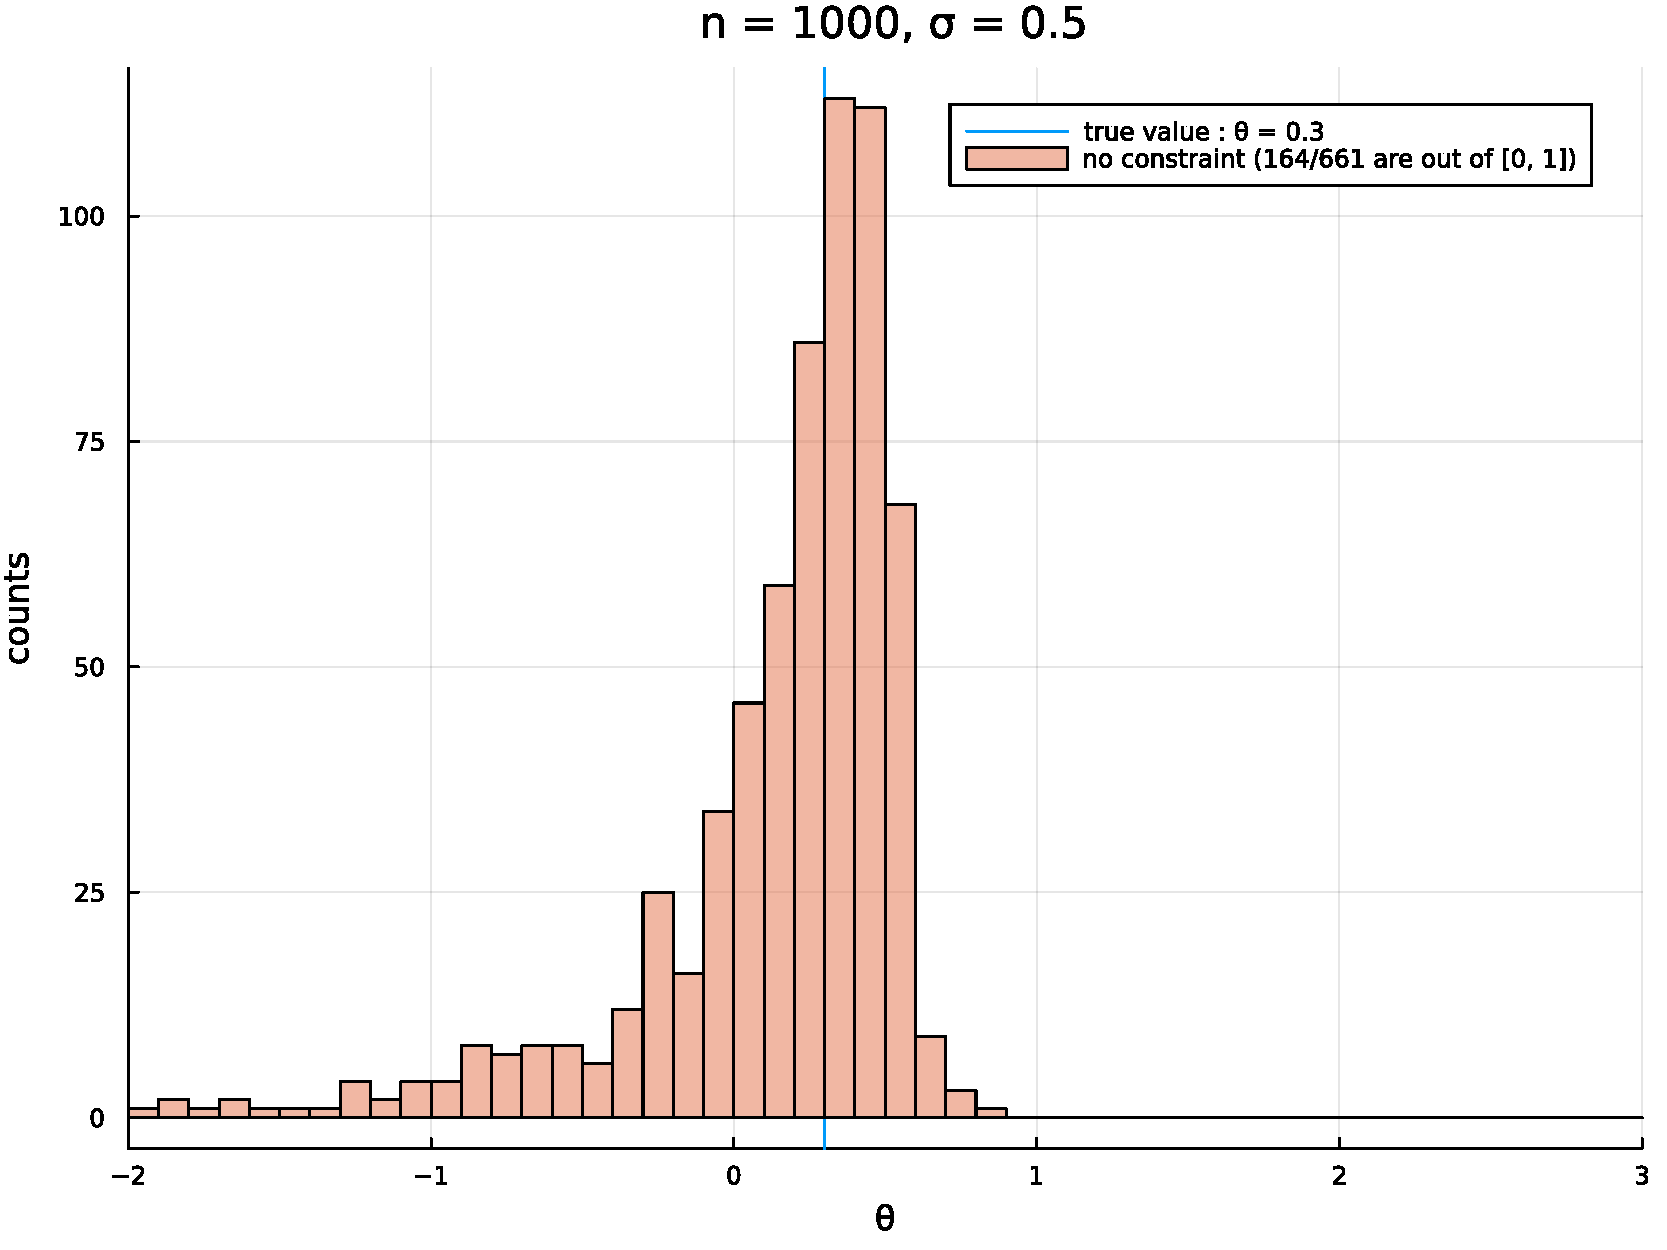
\includegraphics[width = 0.5\textwidth]
  {figuretable/histogram_loglinear_loglinear_n_1000_sigma_0.5_non_constraint.pdf}}
  \subfloat[]{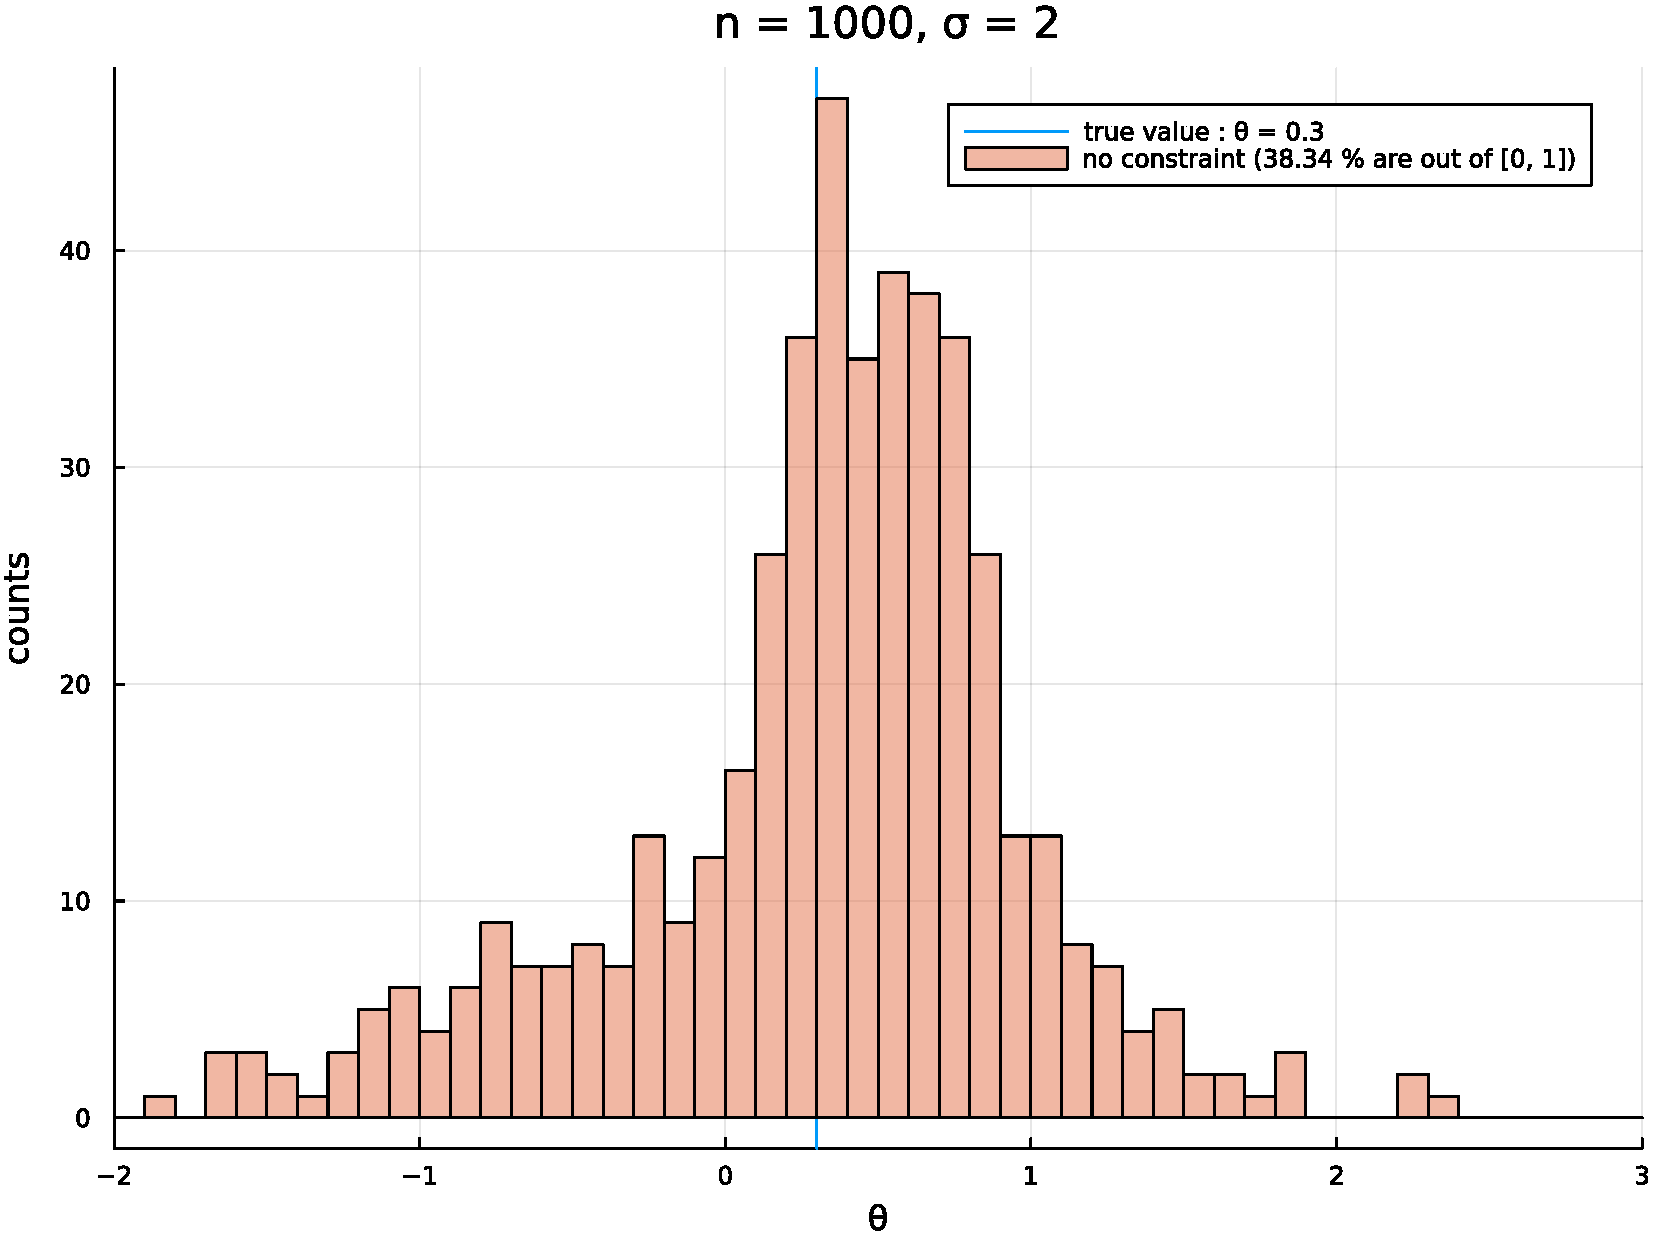
\includegraphics[width = 0.5\textwidth]
  {figuretable/histogram_loglinear_loglinear_n_1000_sigma_2_non_constraint.pdf}}
  \caption{Histograms of the estimation result of the conduct parameter.}
  \label{fg:histogram_loglinear_loglinear_no_constraint} 
  \end{center}
  \footnotesize
  Note: True parameters: $\alpha_1 = \alpha_3 = \gamma_0 = \gamma_1 = \gamma_2  = \gamma_3 = 1, \alpha_0 = 10, \alpha_2 = 0.1,  \theta = 0.3.$
\end{figure}



\section{A problem in log-linear demand specification}

\begin{figure}[!htbp]
  \begin{center}
  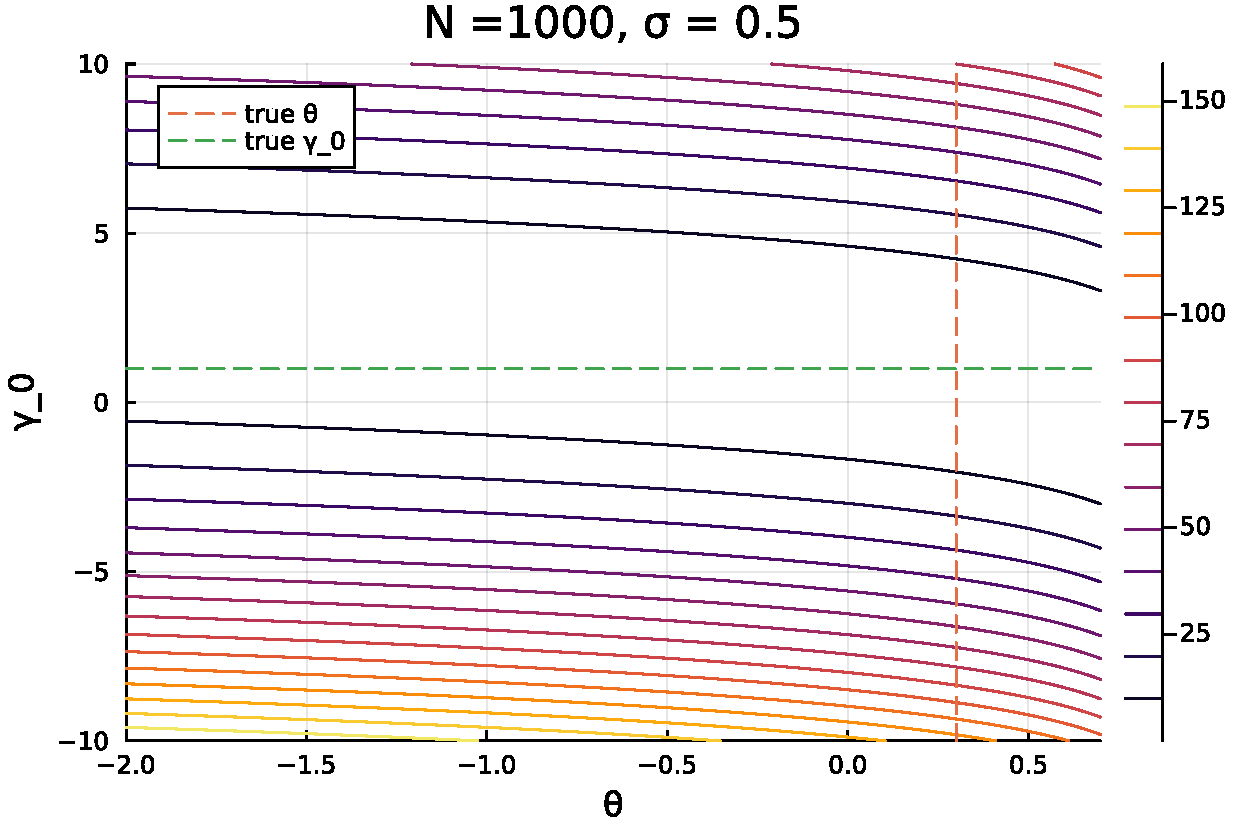
\includegraphics[width = 0.45\textwidth]
  {figuretable/contour_loglinear_loglinear_n_1000_sigma_0.5.pdf}
  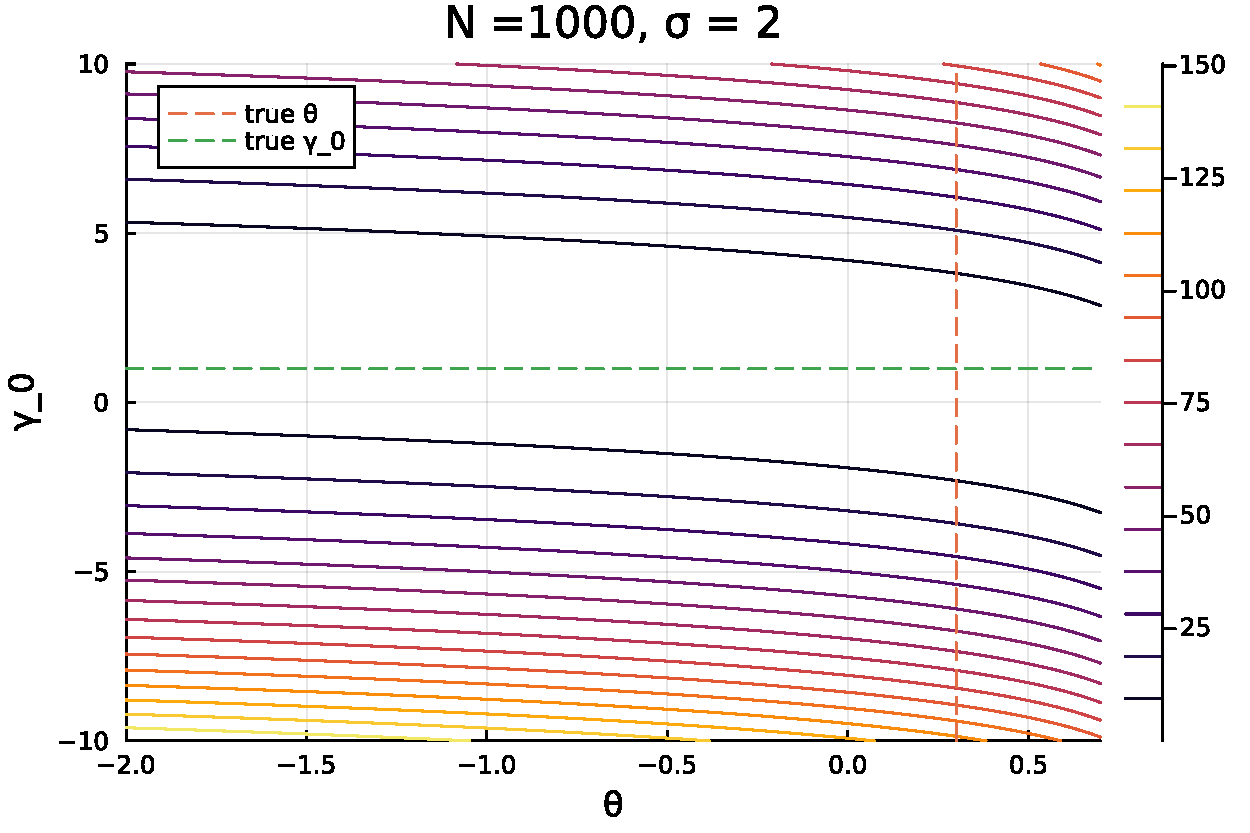
\includegraphics[width = 0.45\textwidth]
  {figuretable/contour_loglinear_loglinear_n_1000_sigma_2.pdf}
  \caption{Contour map of GMM objective function}
  \label{fg:contour_loglinear_loglinear_n_1000_sigma_2} 
  \end{center}
  \footnotesize
  Note: True parameters: $\alpha_1 = \alpha_3 = \gamma_0 = \gamma_1 = \gamma_2  = \gamma_3 = 1, \alpha_0 = 10, \alpha_2 = 0.1,  \theta = 0.3.$
\end{figure} 

First, note that in Table \ref{tb:loglinear_loglinear_non_constraint}, the mean of $\gamma_0$, the constant term in the log-linear marginal cost function, is far from the true parameter and the standard deviation is large compared with other marginal cost parameters. 
Recall that the first and second term in the supply equation \eqref{eq:log_linear_supply_equation} is $-\log(1 - \theta(\alpha_1 + \alpha_2 Z^{R}_{t})) + \gamma_0$.
As the first term is always negative, for any value of $\theta$ that satisfies $1 - \theta(\alpha_1 + \alpha_2 Z^{R}_{t})$, we can find a value of $\gamma_0$ that cancel out the first and the second term each other.
Especially when the other estimated parameters are close to the true value, by adjusting the value of $\theta$ and $\gamma_0$ to cancel out the first and second term, we can make the value of the GMM objective function under the estimated parameters close to the value of the GMM objective function under the true parameter.

Figure \ref{fg:contour_loglinear_loglinear_n_1000_sigma_2} illustrates the contour map of the GMM objective function with respect to $\gamma_0$ and $\theta$ for one typical data.
To draw the map, we fix the other demand and cost parameter values to the true values and set the grid size to 0.01.
We can see that the contour map has a flat region around the true parameters.
Especially, even though we vary the value of $\theta$, the GMM value does not change around the true value of $\gamma_0$.

As we reported in Section \ref{subsec:log_linear_demand_and_log_linear_marginal_cost}, the value of the estimator of the conduct parameter can take very large or small values.
Do such values minimize the value of the GMM objective function?
To check this, for each simulation, we compute (1) the absolute differences between the true and estimated values of $\theta$ and $\gamma_0$ and (2) the absolute differences between the value of the GMM objective function under the true and estimated parameter.
Figure \ref{fg:diff_gmm_loglinear_loglinear} shows the plot of these differences. 
Each dot corresponds to each simulation and the color of each dot represents the value of the difference in the GMM objective function. 
The darker a dot is, the smaller the difference is.
We expect that when the difference between the true parameter value and the estimation result is small, the difference in the value of the GMM function is small, which implies that the color of the dot is darker. 
However, we can see dark dots even when the difference in the conduct parameter is large.
For example, when $\sigma = 0.5$, dark dots appear when the difference is more than 10.
When $\sigma = 2$, dark dots appear even when the difference is more than 20.
While \citet{lau1982identifying} shows the joint identification result of the conduct parameter and the cost parameter in a general case, Figures \ref{fg:contour_loglinear_loglinear_n_1000_sigma_2} and \ref{fg:diff_gmm_loglinear_loglinear} imply that the estimation of the conduct parameter and the cost parameter becomes imprecise.


\begin{figure}[!htbp]
  \begin{center}
  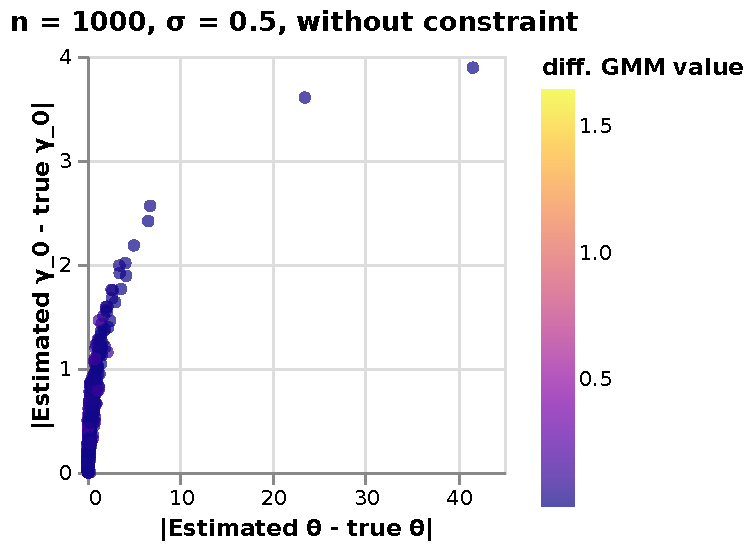
\includegraphics[width = 0.45\textwidth]
  {figuretable/diff_gmm_value_loglinear_loglinear_n_1000_sigma_0.5_non_constraint.pdf}
  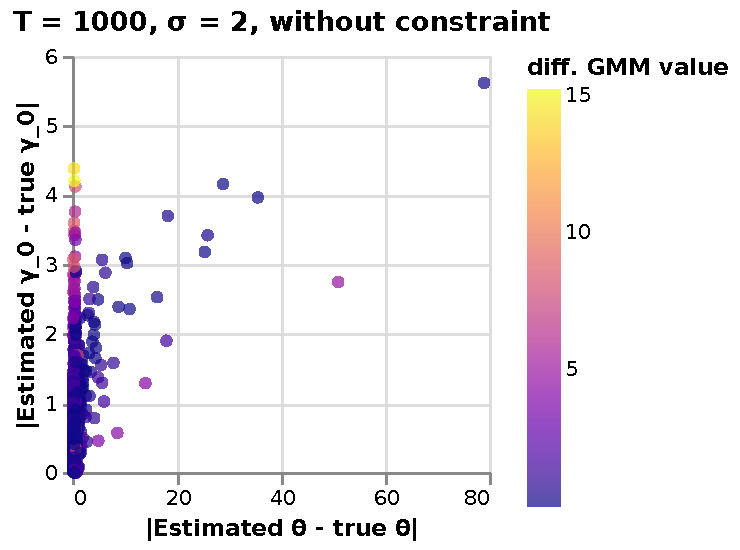
\includegraphics[width = 0.45\textwidth]
  {figuretable/diff_gmm_value_loglinear_loglinear_n_1000_sigma_2_non_constraint.pdf}
  \caption{The difference of the GMM objective function under true parameter and the estimation result}
  \label{fg:diff_gmm_loglinear_loglinear} 
  \end{center}
  \footnotesize
  Note: The x-axis is the difference between the values of the true and estimated conduct parameter. The y-axis is the difference between the values of estimated and true $\gamma_0$. Each dot represents the value of the difference of the GMM objective function under the true and estimated values of the parameters. 
\end{figure} 

The next question is whether we can obtain accurate results by imposing the parameter constraint, that is, $\theta \in [0,1]$.
Our conclusion is no.

Figure \ref{fg:histogram_loglinear_loglinear_with_constraint} overlaps the histograms of the result of the conduct parameter estimation with the parameter constraint on Figure \ref{fg:histogram_loglinear_loglinear_no_constraint}.
For the values in $(0,1)$, the shape of the histograms is similar, but we can see the spike around $\theta = 0$ and $1$.
This is simply because all estimation results out of the bound in the estimation without constraint are gathered at the corner points of the constraint.
The literature interprets $\theta = 0$ and $1$ as perfect competition and collusion, respectively.
Thus, putting the parameter constraint on the conduct parameter makes researchers misinterpret that the markets are perfectly competitive or collusive.
For example, \cite{merel2009measuring} uses log-linear models and the estimated $\theta$ is 0.002 with 0.007 standard error, which means perfect competitive markets. 
The estimation may fail in the boundary as in Figure \ref{fg:histogram_loglinear_loglinear_with_constraint}. 

In summary, the suggestion of the log-linear model in \cite{perloff2012collinearity} adds another problem in its estimation. 
We conclude that at least the linear model can achieve a proper estimation of the conduct parameter in homogeneous good markets. 



\begin{figure}[!htbp]
  \begin{center}
  \subfloat[]{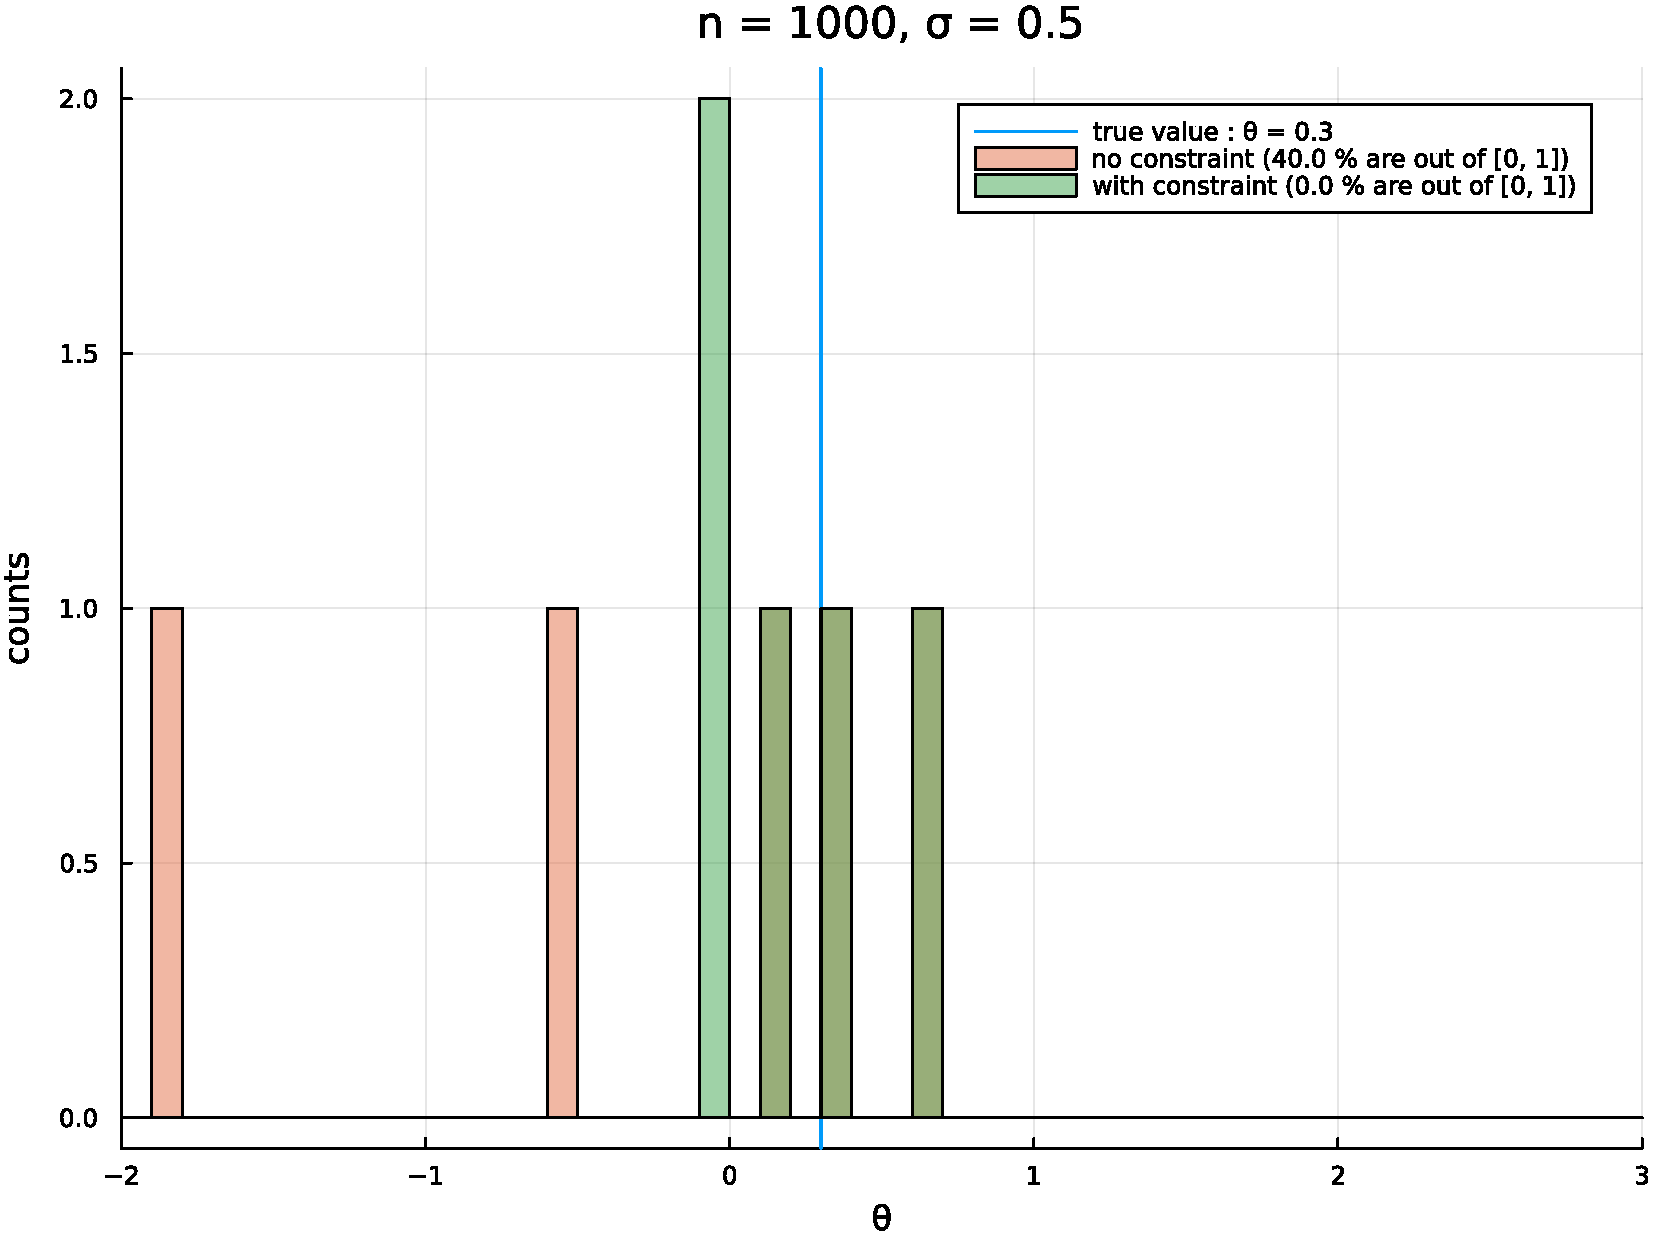
\includegraphics[width = 0.5\textwidth]
  {figuretable/histogram_loglinear_loglinear_n_1000_sigma_0.5_theta_constraint.pdf}}
  \subfloat[]{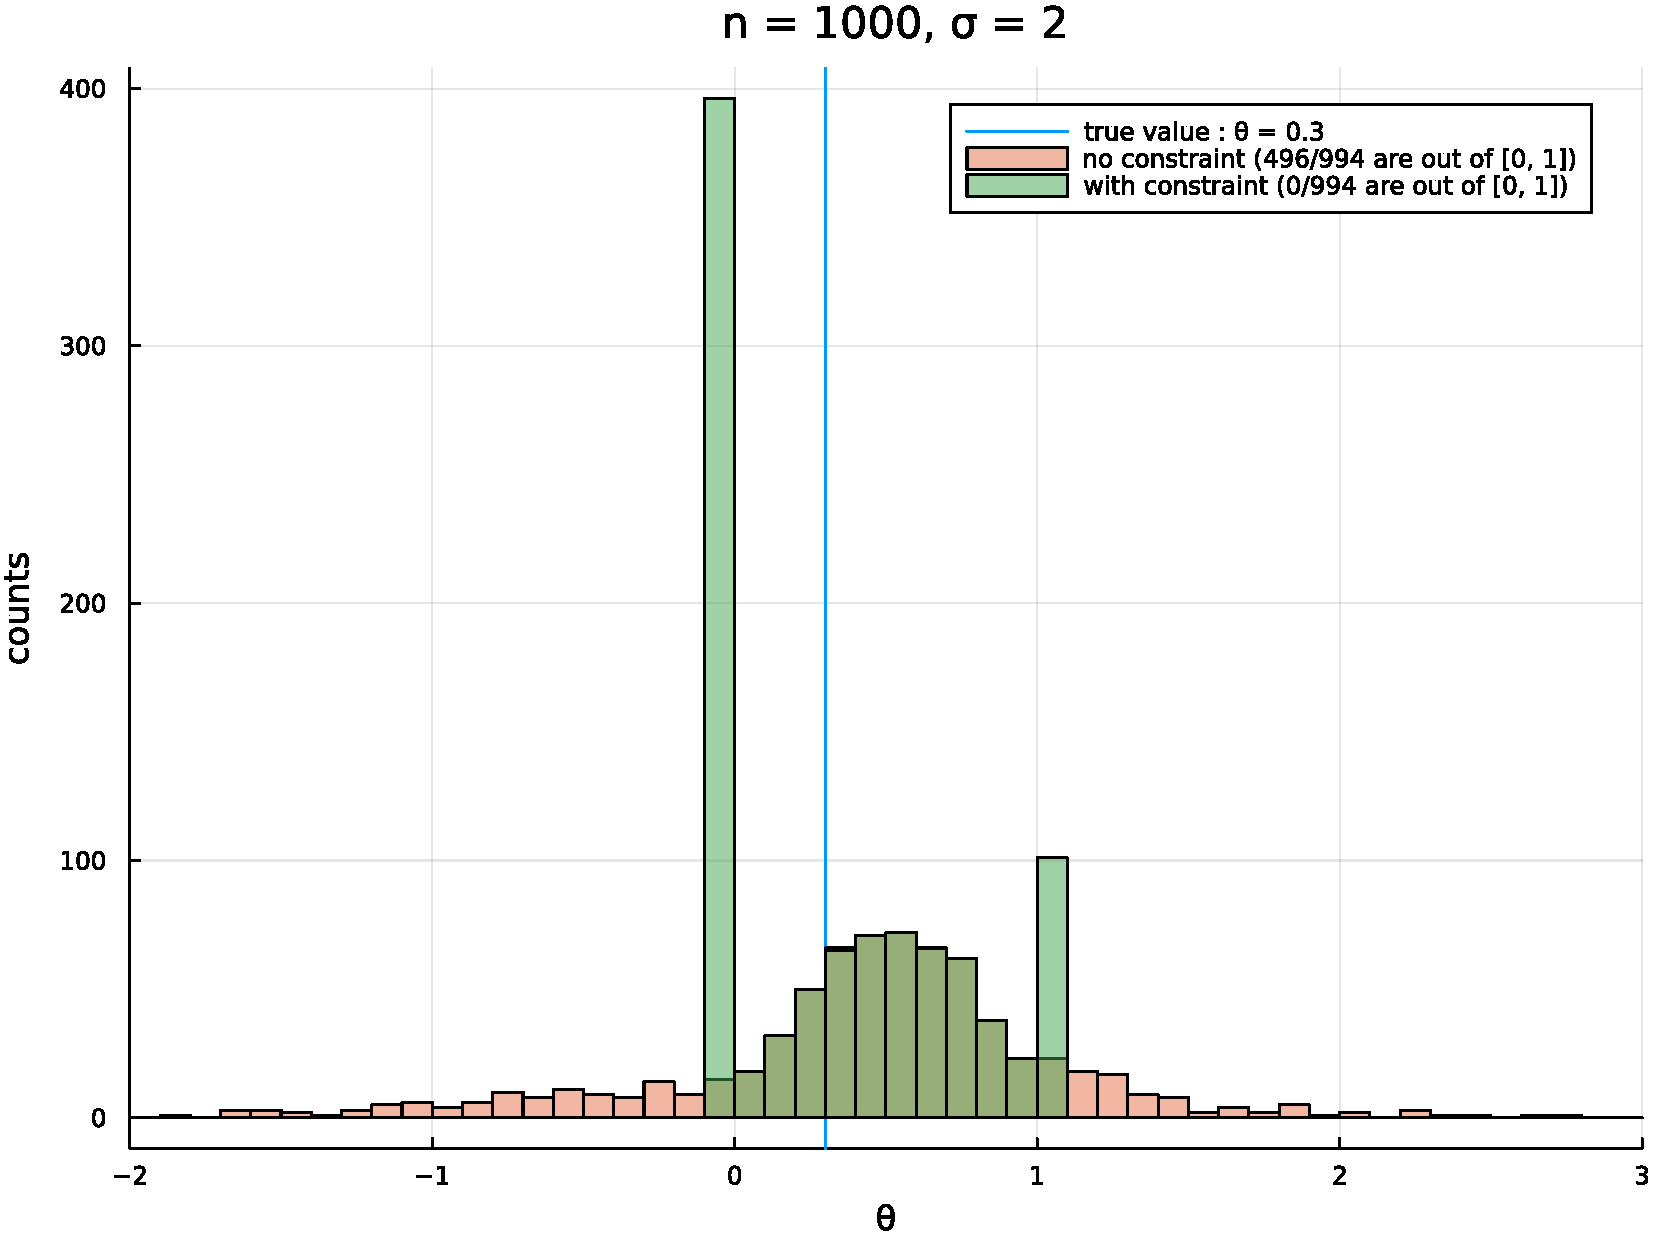
\includegraphics[width = 0.5\textwidth]
  {figuretable/histogram_loglinear_loglinear_n_1000_sigma_2_theta_constraint.pdf}}
  \caption{Histograms of the conduct parameter with and without constraint.}
  \label{fg:histogram_loglinear_loglinear_with_constraint} 
  \end{center}
  \footnotesize
  Note: True parameters: $\alpha_1 = \alpha_3 = \gamma_0 = \gamma_1 = \gamma_2  = \gamma_3 = 1, \alpha_0 = 10, \alpha_2 = 0.1,  \theta = 0.3.$
\end{figure}




    
\section{Conclusion}
We revisit the conduct parameter estimation in homogeneous goods markets. In contrast to the pessimistic simulation results shown in \cite{perloff2012collinearity}, our simulation shows that the estimation becomes accurate by properly adding demand shifters in the supply estimation and increasing the sample size. We also show that the log-linear model recommended by \cite{perloff2012collinearity} has another estimation problem. Based on the numerical investigation, we conclude that at least the linear model can achieve a proper estimation of the conduct parameter in homogeneous good markets.


\bibliographystyle{aer}
\bibliography{conduct_parameter}


\end{document}